\documentclass[convert={density=1200,size=20000x20000,outext=.png}]{standalone}

\usepackage{tikz}
\usetikzlibrary{arrows}
\usetikzlibrary{decorations.markings}
\usetikzlibrary{calc}
\usetikzlibrary{decorations.text}

\begin{document}

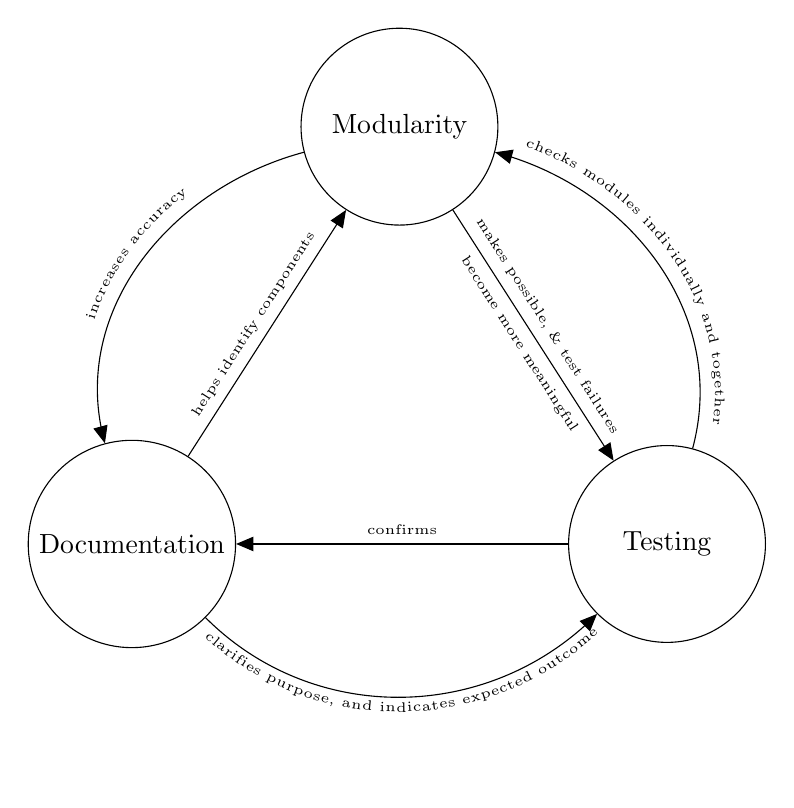
\begin{tikzpicture}

\def\downshift#1{\raisebox{-2.5ex}}
\def\upshift#1{\raisebox{2.5ex}}

\draw[draw=none, fill=white] (-4.5, -4.5) rectangle (4.5, 4.5);

\node[circle, draw=black, fill=white, minimum size=2.5cm] (M) at (0, 3.8) {Modularity};
\node[circle, draw=black, fill=white, minimum size=2.5cm] (D) at (-3.398075, -1.5) {Documentation};
\node[circle, draw=black, fill=white, minimum size=2.5cm] (T) at (3.398075, -1.5) {Testing};

\draw[-triangle 45] (M) -- (T) node[pos=0.5, sloped, align=center] {\tiny makes possible, \& test failures\\\tiny become more meaningful};
\draw[triangle 45-] (D) edge[out=105,in=195, postaction={decorate,decoration={text along path,text align=center,text={|\tiny\upshift|increases accuracy}}}] (M);
\draw[-triangle 45] (D) edge[out=-45,in=-135, postaction={decorate,decoration={text along path,text align=center,text={|\tiny\downshift|clarifies purpose, and indicates expected outcome}}}] (T);
\draw[-triangle 45] (D) -- (M) node[pos=0.5, sloped, above, align=center] {\tiny helps identify components};
\draw[triangle 45-] (M) edge[out=-15,in=75, postaction={decorate,decoration={text along path,text align=center,text={|\tiny\upshift|checks modules individually and together}}}] (T);
\draw[-triangle 45] (T) -- (D) node[pos=0.5, above] {\tiny confirms};

\end{tikzpicture}

\end{document}
